\section{Optimal Transport}%
\label{sec:optimal-transport}
\vspace{0.5cm}
\begin{figure}[h!]%
  \label{fig:escher}
  \centering
  \fcolorbox{black}{white}{
    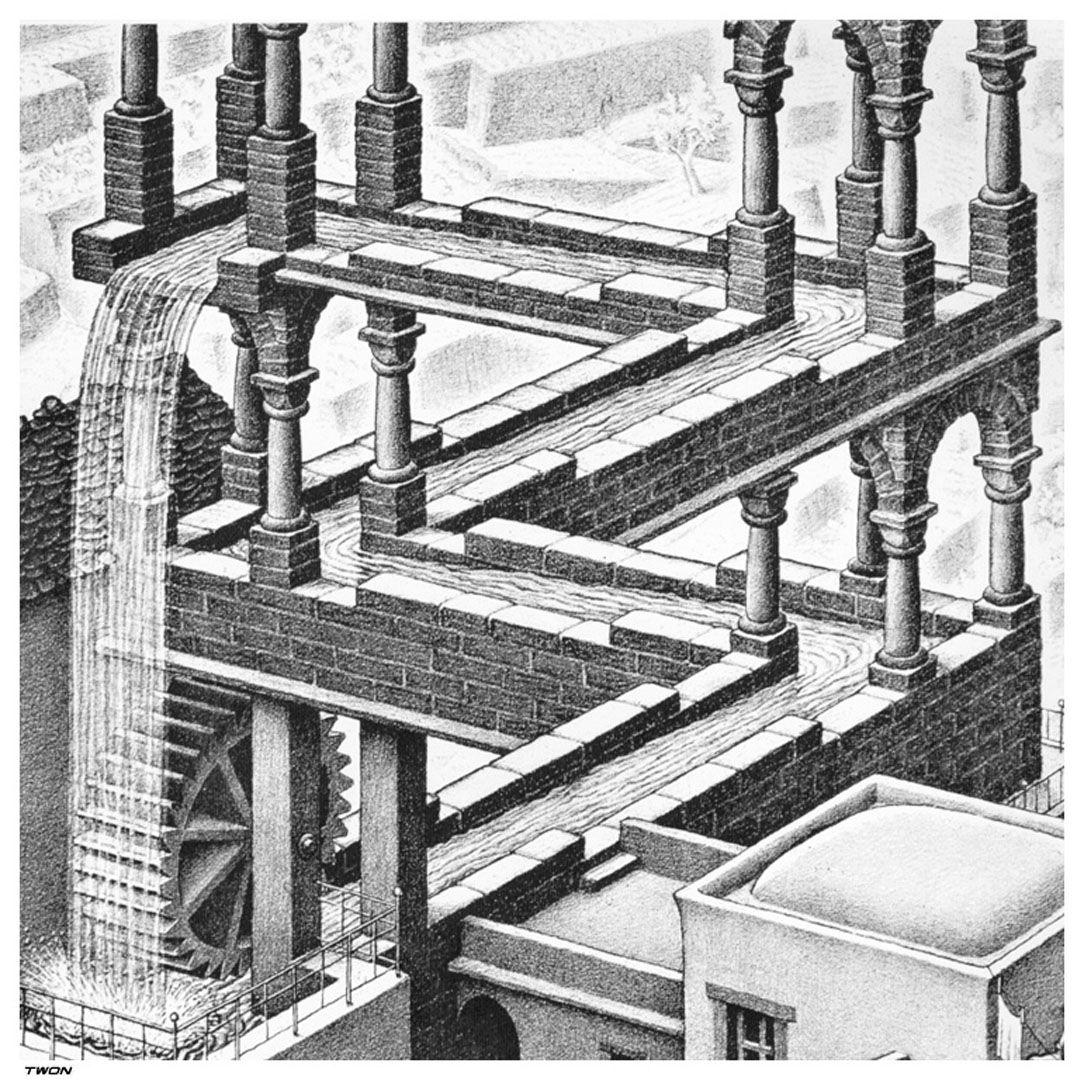
\includegraphics[width=0.3\textwidth]{escher}
  }
  \caption{M.C. Escher, ``Waterfall'', 1961. This impossible construction illustrates the challenges of measuring distance in complex spaces, analogous to the difficulties in comparing probability distributions with divergences that have discontinuities.}
\end{figure}
\vspace{0.5cm}

In Section~\ref{sec:information-theory}, we explored how the GAN generator minimizes an approximation of the Jensen-Shannon divergence between the real data distribution $p_{data}$ and the generated distribution $p_g$. However, this approach suffers from fundamental limitations rooted in the topology induced by the Jensen-Shannon divergence. In this section, we examine these limitations and introduce optimal transport theory as a more robust framework for comparing probability distributions, leading to the Wasserstein GAN (WGAN) variant.

The central insight is that the choice of distance metric has profound consequences for continuity and convergence properties of probability distributions. As we will see, the Wasserstein distance provides a more suitable topology for GAN training, addressing key limitations of the original formulation.

\subsection{Topology and Convergence of Probability Distributions}

To understand the limitations of the original GAN formulation, we first need to examine how different metrics induce different topologies on spaces of probability distributions.

\begin{definition}%
  \label{def:topology1}
  Let $\mathcal{X}$ be any set. A \textnormal{\sffamily topology} $\mathcal{T}$ on $\mathcal{X}$ is a collection of subsets of $\mathcal{X}$ (called \textnormal{\sffamily open sets}) satisfying:
  \begin{enumerate}[(i)]
    \item The empty set and $\mathcal{X}$ itself are open;
    \item The intersection of finitely many open sets is open;
    \item The union of any collection of open sets is open.
  \end{enumerate}
  The pair $(\mathcal{X}, \mathcal{T})$ is called a \textnormal{\sffamily topological space}.
\end{definition}

In metric spaces, the topology is generated by open balls, which form a basis for the topology.

\begin{definition}%
  \label{def:open-ball}
  Let $(\mathcal{X}, d)$ be a metric space. An \textnormal{\sffamily open ball} of radius $r > 0$ centered at $x_0 \in \mathcal{X}$ is:
  \begin{align}
    B_d(x_0, r) = \{ x \in \mathcal{X} : d(x, x_0) < r \}.
  \end{align}
\end{definition}

\begin{definition}%
  \label{def:topology2}
  Let $(\mathcal{X}, d)$ be a metric space. The \textnormal{\sffamily topology induced by} $d$ is the topology generated by the basis of open balls $\mathcal{B} = \{B_d(x, r) \mid x \in \mathcal{X}, r > 0\}$.
\end{definition}

Different metrics can induce different topologies with varying degrees of "granularity" or "fineness."

\begin{theorem}%
  \label{thm:granularity}
  Let $d$ and $d'$ be metrics on $\mathcal{X}$, with induced topologies $\mathcal{T}$ and $\mathcal{T}'$. Then $\mathcal{T}'$ is \textnormal{\sffamily finer} than $\mathcal{T}$ if and only if for every $x \in \mathcal{X}$ and $\epsilon > 0$, there exists $\delta > 0$ such that $B_{d'}(x, \delta) \subset B_d(x, \epsilon)$.
\end{theorem}

For probability distributions, convergence depends on the chosen metric:

\begin{definition}%
  \label{def:convergence-metric-space}
  Let $\mathcal{P}$ be the space of probability distributions on $\mathcal{X}$ with equal support, and let $d: \mathcal{P} \times \mathcal{P} \to \mathbb{R}$ be a metric. A sequence $\{P_n\}_{n \in \mathbb{N}}$ \textnormal{\sffamily converges} to $P$ if $d(P_n, P) \to 0$ as $n \to \infty$.
\end{definition}

The Kullback-Leibler and Jensen-Shannon divergences induce a coarser topology than the Wasserstein distance, meaning they have fewer open sets and stronger requirements for convergence. This coarser topology leads to discontinuities that cause problems in GAN training.

\subsection{Limitations of KL and Jensen-Shannon Divergences}

The Kullback-Leibler (KL) and Jensen-Shannon (JS) divergences, while useful in many contexts, have significant limitations when comparing distributions with disjoint supports—a common scenario in GAN training.

\begin{example}[Learning Parallel Lines]
  \label{example:learning-parallel-lines}
  Consider learning to generate a vertical line at $x=0$ when starting from a line at $x=\phi$. Let $\mathcal{X} = \mathbb{R}^2$, $p_0(z)$ be the uniform distribution over $\{(0, z) : z \in [0, 1]\}$, and $G_\phi(z)$ generate points $\{(\phi, z) : z \in [0, 1]\}$. We want to train $G_\phi$ to approximate $p_0$ by moving $\phi \to 0$.
  
  \begin{figure}[h]
    \centering
    \begin{tikzpicture}[scale=2,>=stealth]
      \draw[line] (-1,-0.5) rectangle (2,2);
      \draw[red, thick, ->] (0,0) -- (0,1);
      \draw[blue, thick, ->] (1,0) -- (1,1);
      \draw[dotted] (-0.8,0) -- (1.8,0) node[anchor=north east]{$x$};
      \draw[dotted] (0,-0.3) -- (0,1.8) node[anchor=north east]{$y$};
      \draw (0,0) node[anchor=north east]{$(0,z)$};
      \draw (1,0) node[anchor=north east]{$(\phi,z)$};
    \end{tikzpicture}
    \caption{Parallel lines example: the target distribution (red) and generator distribution (blue) have disjoint supports when $\phi \neq 0$.}%
    \label{fig:parallel-lines}
  \end{figure}
  
  \begin{enumerate}[(i)]
    \item \textbf{KL Divergence:} For $\phi \neq 0$, the distributions have disjoint supports:
    \begin{align}
      \text{KL}(p_0 \| G_\phi) = \mathbb{E}_{z \sim p_0} \left[ \log \frac{p_0(z)}{G_\phi(z)} \right] = \infty
    \end{align}
    since $G_\phi(z) = 0$ for all $z \sim p_0$. Similarly, $\text{KL}(G_\phi \| p_0) = \infty$. Only when $\phi = 0$ do we have $\text{KL}(p_0 \| G_\phi) = 0$.
    
    \item \textbf{Jensen-Shannon Divergence:} The JS divergence also fails to provide a useful gradient:
    \begin{align}
      \text{JSD}(p_0 \| G_\phi) &= \frac{1}{2} \mathbb{E}_{z \sim p_0} \left[ \log \frac{p_0(z)}{p_m(z)} \right] + \frac{1}{2} \mathbb{E}_{z \sim G_\phi} \left[ \log \frac{G_\phi(z)}{p_m(z)} \right] \\
      &= \frac{1}{2} \mathbb{E}_{z \sim p_0} [\log 2] + \frac{1}{2} \mathbb{E}_{z \sim G_\phi} [\log 2] \\
      &= \log 2
    \end{align}
    where $p_m = \frac{p_0 + G_\phi}{2}$. Again, this is constant ($\log 2$) for all $\phi \neq 0$ and only drops to 0 when $\phi = 0$.
  \end{enumerate}
\end{example}

This example illustrates a fundamental problem: both KL and JS divergences provide no useful gradient information when distributions have disjoint supports, which is common in high-dimensional spaces like those used in GANs.

\subsection{The Manifold Hypothesis and Dimensionality}

In practice, GANs often operate on high-dimensional data like images, where the data lies on low-dimensional manifolds embedded in the ambient space.

\begin{definition}
  A \textnormal{\sffamily manifold} is a topological space that locally resembles Euclidean space near each point. Formally, an $n$-dimensional manifold is a topological space where each point has a neighborhood homeomorphic to $\mathbb{R}^n$.
\end{definition}

\begin{remark}[Manifold Hypothesis]
  The \textnormal{\sffamily manifold hypothesis} posits that real-world high-dimensional data (such as images) lie on low-dimensional manifolds embedded in the ambient space. For example, the space of all possible $H \times W$ RGB images is $[0, 255]^{3 \times H \times W}$, but natural images occupy only a tiny fraction of this space.
\end{remark}

This phenomenon is related to the \textit{curse of dimensionality}~\cite{ref:bellman-1957}: as dimensionality increases, the volume of the space grows exponentially, making data increasingly sparse. For instance, covering a unit interval with points spaced 0.1 units apart requires 10 points; covering a unit square requires 100 points; a unit cube requires 1000 points, and so on.

In GANs, the generator and real data distributions typically lie on different low-dimensional manifolds within the high-dimensional ambient space. When these manifolds are disjoint (which is likely in high dimensions), the KL and JS divergences become constant or infinite, providing no useful gradient signal.

\subsection{The Perfect Discriminator Problem}

The limitations of KL and JS divergences lead to a critical issue in GAN training: the emergence of a "perfect discriminator" that halts learning.

\begin{definition}%
  \label{def:perfect-discriminator}
  A \textnormal{\sffamily perfect discriminator} is a function $D: \mathcal{X} \to [0,1]$ that achieves perfect accuracy on both real and generated data:
  \begin{align}
    \mathbb{P}_{x \sim p_{data}}(\{x : D(x) = 1\}) &= 1, \\
    \mathbb{P}_{\tilde{x} \sim p_g}(\{\tilde{x} : D(\tilde{x}) = 0\}) &= 1.
  \end{align}
\end{definition}

\begin{theorem}%
  \label{thm:perfect-discriminator}
  If $D$ is a perfect discriminator, then $\nabla_\phi V = 0$, meaning the generator receives no gradient signal and learning stops.
\end{theorem}
\begin{proof}
  The generator update is:
  \begin{align}
    \phi^{(t+1)} &\gets \phi^{(t)} - \alpha \nabla_\phi \frac{1}{m} \sum_{i=1}^m \log(1 - D^{(t+1)}(G_{\phi^{(t)}}(z_i))) \\
    &\gets \phi^{(t)} - \alpha \nabla_\phi \frac{1}{m} \sum_{i=1}^m \log(1 - 0) \\
    &\gets \phi^{(t)} - \alpha \nabla_\phi \frac{1}{m} \sum_{i=1}^m \log(1) \\
    &\gets \phi^{(t)}
  \end{align}
  Thus, the generator parameters do not update.
\end{proof}

\begin{theorem}%
  \label{thm:too-early}
  If $D$ becomes a perfect discriminator early in training, then $D$ also stops learning, as its gradients vanish.
\end{theorem}
\begin{proof}
  The discriminator update is:
  \begin{align}
    \theta^{(t+1)} &\gets \theta^{(t)} - \alpha \nabla_\theta \frac{1}{m} \sum_{i=1}^m \left[ \log D^{(t)}(x_i) + \log(1 - D^{(t)}(G_{\phi^{(t)}}(z_i))) \right] \\
    &\gets \theta^{(t)} - \alpha \nabla_\theta \frac{1}{m} \sum_{i=1}^m \left[ \log(1) + \log(1) \right] \\
    &\gets \theta^{(t)}
  \end{align}
  Thus, the discriminator parameters also do not update.
\end{proof}

This perfect discriminator problem illustrates a fundamental limitation of the original GAN formulation: once the discriminator becomes too good too quickly, training stalls completely. We need a "gentler" discriminator that provides meaningful gradients throughout training.

\subsection{Optimal Transport Theory}

Optimal transport theory provides a more robust framework for comparing probability distributions, addressing the limitations of KL and JS divergences. The theory originated with Gaspard Monge in 1781 and was later generalized by Leonid Kantorovich.

\begin{definition}%
  \label{def:transport-plan}
  Let $\mathcal{X}$ and $\mathcal{Y}$ be spaces, and let $p$ and $q$ be probability distributions on $\mathcal{X}$ and $\mathcal{Y}$, respectively. A \textnormal{\sffamily transport plan} is a joint probability distribution $\gamma \in \Gamma(p, q)$, where $\Gamma(p, q) = \{\gamma : \gamma \text{ has marginals } p \text{ and } q\}$. The set $\Gamma(p, q)$ is called the \textnormal{\sffamily set of couplings} between $p$ and $q$.
\end{definition}

\begin{remark}
  Each transport plan $\gamma(x, y)$ represents the amount of "mass" to move from $x$ to $y$ to transform distribution $p$ into distribution $q$.
\end{remark}

\begin{definition}%
  \label{def:transport-cost}
  Given a cost function $c: \mathcal{X} \times \mathcal{Y} \to \mathbb{R}^+$, the \textnormal{\sffamily transport cost} of plan $\gamma$ is:
  \begin{align}
    \mathbb{E}_{(x,y) \sim \gamma}[c(x, y)] = \int_{\mathcal{X}} \int_{\mathcal{Y}} c(x, y) \, d\gamma(x, y)
  \end{align}
  For the $p$-Wasserstein distance, we use $c(x, y) = \|x - y\|^p$.
\end{definition}

The goal of optimal transport is to find the transport plan with minimal cost:

\begin{definition}%
  \label{def:wasserstein}
  The \textnormal{\sffamily $p$-Wasserstein distance} between distributions $p$ and $q$ is:
  \begin{align}
    W_p(p, q) = \left( \inf_{\gamma \in \Gamma(p, q)} \mathbb{E}_{(x,y) \sim \gamma}[\|x - y\|^p] \right)^{1/p}
  \end{align}
  For $p = 1$, we call this the \textnormal{\sffamily Kantorovich distance} or \textnormal{\textsf earth mover's distance}.
\end{definition}

The Wasserstein distance provides a more robust metric for comparing distributions, especially when they have disjoint supports.

\begin{example}[Learning Parallel Lines (Revisited)]
  Using the Wasserstein-1 distance for our parallel lines example:
  \begin{align}
    W_1(G_\phi, p_0) &= \inf_{\gamma \in \Gamma(G_\phi, p_0)} \mathbb{E}_{(x,y) \sim \gamma}[\|x - y\|] \\
    &= \inf_{\gamma \in \Gamma(G_\phi, p_0)} \mathbb{E}_{(x,y) \sim \gamma}[\sqrt{(\phi - 0)^2 + (z - z)^2}] \\
    &= |\phi|
  \end{align}
  Unlike KL and JS divergences, the Wasserstein distance provides a continuous, meaningful gradient signal ($\nabla_\phi W_1 = \text{sign}(\phi)$) even when the distributions have disjoint supports.
\end{example}

\subsection{Kantorovich-Rubinstein Duality}

Directly computing the Wasserstein distance is intractable due to the infimum over all possible transport plans. However, the Kantorovich-Rubinstein duality provides an alternative formulation:

\begin{definition}
  A function $f: \mathcal{X} \to \mathbb{R}$ is \textnormal{\sffamily $K$-Lipschitz} if for all $x_1, x_2 \in \mathcal{X}$:
  \begin{align}
    |f(x_1) - f(x_2)| \leq K \cdot d(x_1, x_2)
  \end{align}
  where $d$ is the metric on $\mathcal{X}$.
\end{definition}

\begin{theorem}[Kantorovich-Rubinstein Duality]
  \label{thm:kr-duality}
  The 1-Wasserstein distance can be expressed as:
  \begin{align}
    W_1(p, q) = \sup_{f \in \mathcal{F}} \left( \mathbb{E}_{x \sim p}[f(x)] - \mathbb{E}_{x \sim q}[f(x)] \right)
  \end{align}
  where $\mathcal{F}$ is the set of all 1-Lipschitz functions.
\end{theorem}

This dual formulation is computationally more tractable and forms the basis of the Wasserstein GAN. Instead of directly minimizing the Wasserstein distance, we can train a neural network to approximate the optimal 1-Lipschitz function.

\subsection{Wasserstein GAN}

The Wasserstein GAN (WGAN)~\cite{ref:arjovsky-2017} leverages the Kantorovich-Rubinstein duality to create a more stable GAN variant. The key insight is to replace the discriminator with a "critic" that approximates the optimal 1-Lipschitz function.

\begin{definition}
  The \textnormal{\sffamily Wasserstein GAN objective} is:
  \begin{align}
    \min_G \max_{f \in \mathcal{F}} \mathbb{E}_{x \sim p_{data}}[f(x)] - \mathbb{E}_{z \sim p_z}[f(G(z))]
  \end{align}
  where $\mathcal{F}$ is the set of 1-Lipschitz functions.
\end{definition}

In practice, we enforce the Lipschitz constraint through weight clipping or gradient penalty, rather than explicitly constraining the function space.

\begin{figure}[H]
  \centering
  \begin{minipage}{0.9\linewidth}
    \begin{algorithm}[H]
      \SetAlgoLined
      \KwIn{Learning rate $\eta > 0$, Clipping parameter $c > 0$, Number of iterations $T > 0$, Critic iterations per generator iteration $K > 0$}
      \KwOut{Trained generator $G$ and critic $f$}
      Initialize critic parameters $\theta$ and generator parameters $\phi$ randomly\;
      \For{$t = 1$ \KwTo $T$}{
        \For{$k = 1$ \KwTo $K$}{
          Sample $\{x_1, \dots, x_m\}$ from real data distribution $p_{data}$\;
          Sample $\{z_1, \dots, z_m\}$ from prior noise distribution $p_z$\;
          Compute critic loss:
          \[
          L = \frac{1}{m} \sum_{i=1}^m f_\theta(x_i) - \frac{1}{m} \sum_{i=1}^m f_\theta(G_\phi(z_i))
          \]
          Update critic parameters: $\theta \gets \theta + \eta \cdot \nabla_\theta L$\;
          Clip critic weights: $\theta \gets \text{clip}(\theta, -c, c)$\;
        }
        Sample $\{z_1, \dots, z_m\}$ from prior noise distribution $p_z$\;
        Compute generator loss:
        \[
        L = -\frac{1}{m} \sum_{i=1}^m f_\theta(G_\phi(z_i))
        \]
        Update generator parameters: $\phi \gets \phi - \eta \cdot \nabla_\phi L$\;
      }
      \caption{Wasserstein GAN Algorithm}
      \label{algo:wgan}
    \end{algorithm}
  \end{minipage}
\end{figure}

\subsection{Discussion and Comparison}

The Wasserstein GAN addresses several key limitations of the original GAN formulation:

\begin{enumerate}
  \item \textbf{Meaningful gradients with disjoint supports:} Unlike KL and JS divergences, the Wasserstein distance provides continuous gradients even when distributions have disjoint supports, as demonstrated in the parallel lines example.
  
  \item \textbf{Better correlation with sample quality:} The Wasserstein distance correlates more closely with the empirical quality of generated samples, providing a more meaningful training signal.
  
  \item \textbf{Improved stability:} WGAN training is generally more stable and less prone to mode collapse than the original GAN formulation.
\end{enumerate}

However, WGAN has its own limitations:

\begin{enumerate}
  \item \textbf{Weight clipping:} The original WGAN uses weight clipping to enforce the Lipschitz constraint, which can lead to optimization issues and capacity limitations.
  
  \item \textbf{Computational cost:} WGAN typically requires more critic updates per generator iteration, increasing computational cost.
  
  \item \textbf{Convergence speed:} While more stable, WGAN may converge more slowly than some improved GAN variants.
\end{enumerate}

Subsequent improvements like WGAN-GP~\cite{ref:gulrajani-2017} replace weight clipping with a gradient penalty, addressing some of these limitations. The fundamental insight remains: by using a weaker metric (the Wasserstein distance) that induces a finer topology, we can achieve more stable and meaningful GAN training.

The Wasserstein GAN exemplifies how deep theoretical understanding can lead to practical improvements in machine learning algorithms. By recognizing the topological limitations of the original GAN formulation and drawing on optimal transport theory, researchers developed a more robust framework that addresses fundamental challenges in generative modeling.

%%% Local Variables:
%%% mode: latex
%%% TeX-master: "../thesis.tex"
%%% End:
